\Aufgabe{YoungDB}

\begin{enumerate}
    \item \emphColB{Kopiere} aus dem Vorlagenordner des Ressourcen-Laufwerks (\emphColB{R:/gy0187/klassen/10x/Vorlagen/}) die Datei \emphColB{YoungDB.exe} in dein \emphColB{Laufwerk H:/}  (alternativ als Download: \url{klassenkarte.de/index.php/tools/youngdb/})
    \item Öffne nun das Programm YoungDB mit einem Doppelklick auf \emphColB{YoungDB.exe}.
    \item Lege ein \emphColB{neues Datenbankmodell an und speichere es} auf deinem Laufwerk H:/. Dieses kann mit einem Klick auf \emph{Modell speichern unter} gespeichert werden und mit \emph{Modell laden} wieder geöffnet werden.
    
    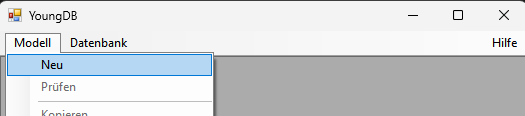
\includegraphics[width=0.4\textwidth]{img/YDB_ModellNeu.png}
    \item Lege \emphColB{zwei neue Klassen} an, bearbeite sie mit \emph{Doppelklick} und erstelle jeweils einen \emphColB{ganzzahligen Primärschlüssel id}.


    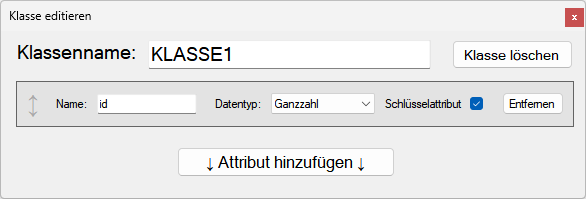
\includegraphics[width=0.5\textwidth]{img/YDB_idErstellen.png}
    \item Erstelle eine Beziehung zwischen den beiden Klassen, indem du mit \emph{Rechtsklick, Halten und Ziehen} eine rote Linie aus einer der Klassen zur anderen ziehst und dann die Maus loslässt. Bearbeite die Beziehung anschließend mit \emph{Doppelklick}, sodass sie eine \emphColB{1:n Beziehung von Klasse2 zu Klasse1} ist.
    
    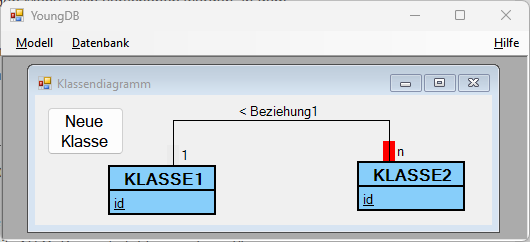
\includegraphics[width=0.5\textwidth]{img/YDB_1nBeziehung.png}
    
    \emph{Tipp:} Klassen kannst du per Doppelklick und \emph{Klasse löschen} entfernen und eine Beziehung, indem du den roten Kasten, der erscheint, wenn deine Maus am Anfang der Linie ist, irgendwo hin ziehst.
    \item \emphColB{Beantworte:} Welche Unterschiede stellst du zu normalen Klassendiagrammen fest?
    
    \LoesungLine{keine Datentypen, }{2}
    \item Erstelle aus dem Modell eine \emphColB{neue Datenbank und speichere sie} auf deinem Laufwerk H:/. Verwende einen ähnlichen Namen wie für das Modell.Hier kannst du Tabellen öffnen, Daten eintragen, SQL-Abfrage schreiben, speichern und laden.
    
    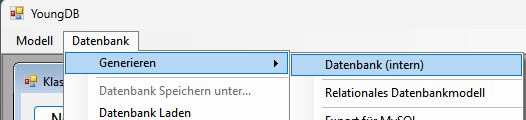
\includegraphics[width=0.45\textwidth]{img/YDB_dbGenerieren.png}
\end{enumerate}



